\section{Sheet stretch}\label{sec:sheet_stretch}


Some information about the following figures. We used a slower stretch speed of 0.001 ps $^{-1}$ = 0.1 \%/ps for these simulations to get more clean figures all though did this not make any noticable changes to the plots of the contact area. We used $T = 5$ K for the vacuum simulation in (in order to reduce vibration) and $T = 300$ K for the contact simulation.

\newpage

% Popup (contact)


\begin{figure}[H]
    \centering
    \begin{subfigure}[b]{0.49\textwidth}
        \centering
        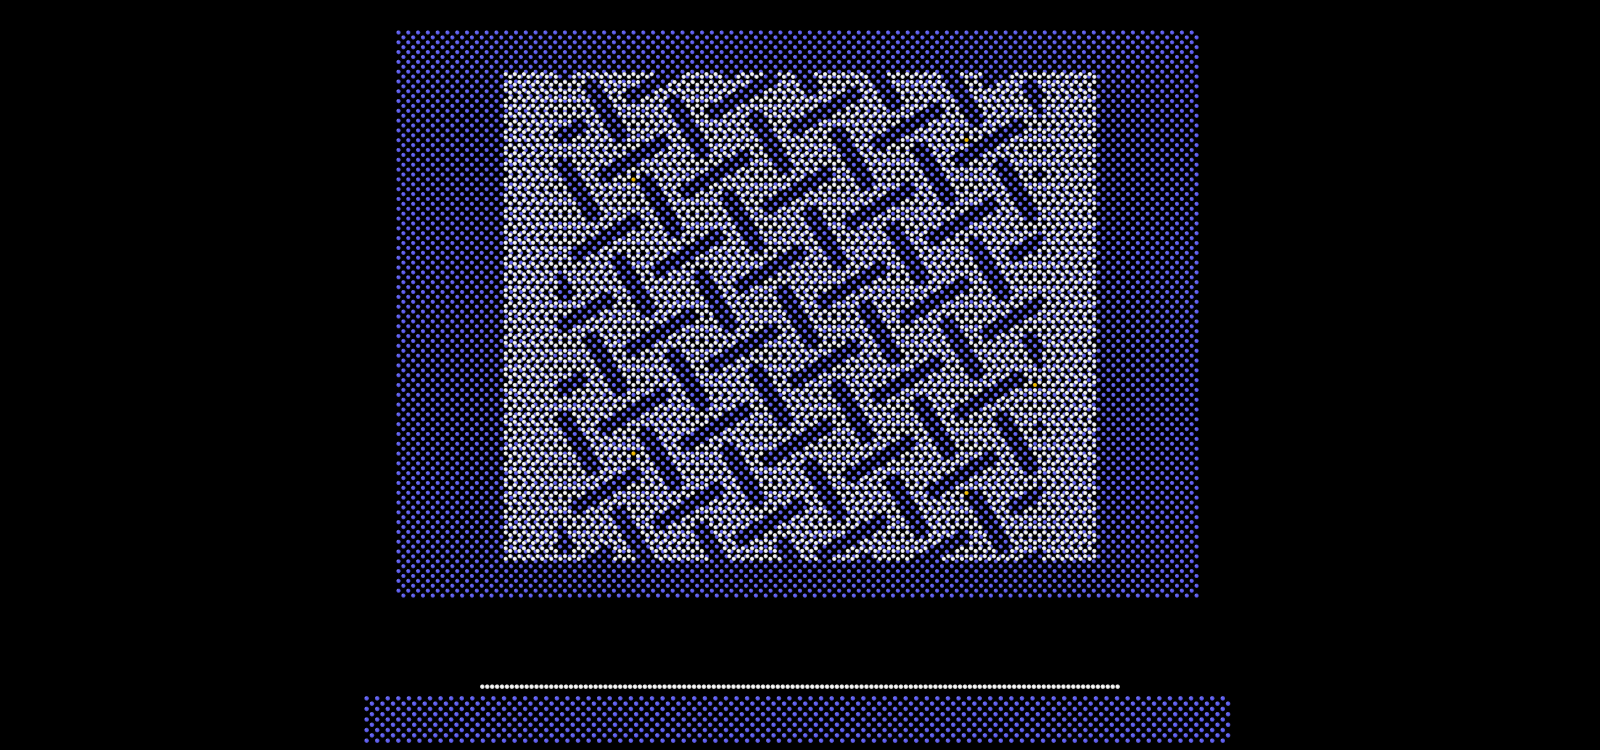
\includegraphics[width=\textwidth]{figures/baseline/contact_vs_stretch/popup/pop_stretch0000.png}
        \caption{Stretch = 0.00}
        \label{fig:}
    \end{subfigure}
    \hfill
    \begin{subfigure}[b]{0.49\textwidth}
        \centering
        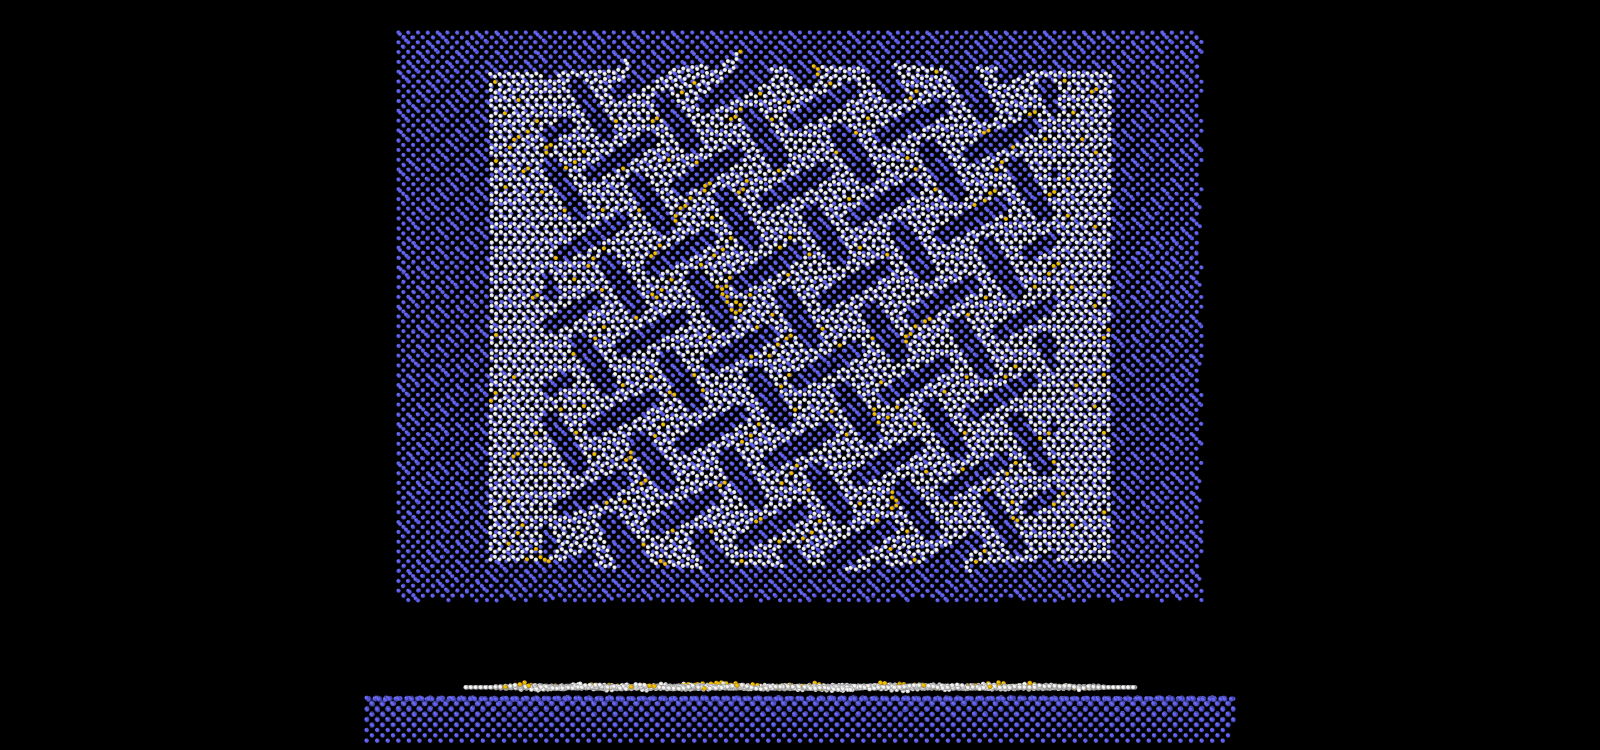
\includegraphics[width=\textwidth]{figures/baseline/contact_vs_stretch/popup/pop_stretch0006.png}
        \caption{Stretch = 0.06}
        \label{fig:}
    \end{subfigure}
    \begin{subfigure}[b]{0.49\textwidth}
        \centering
        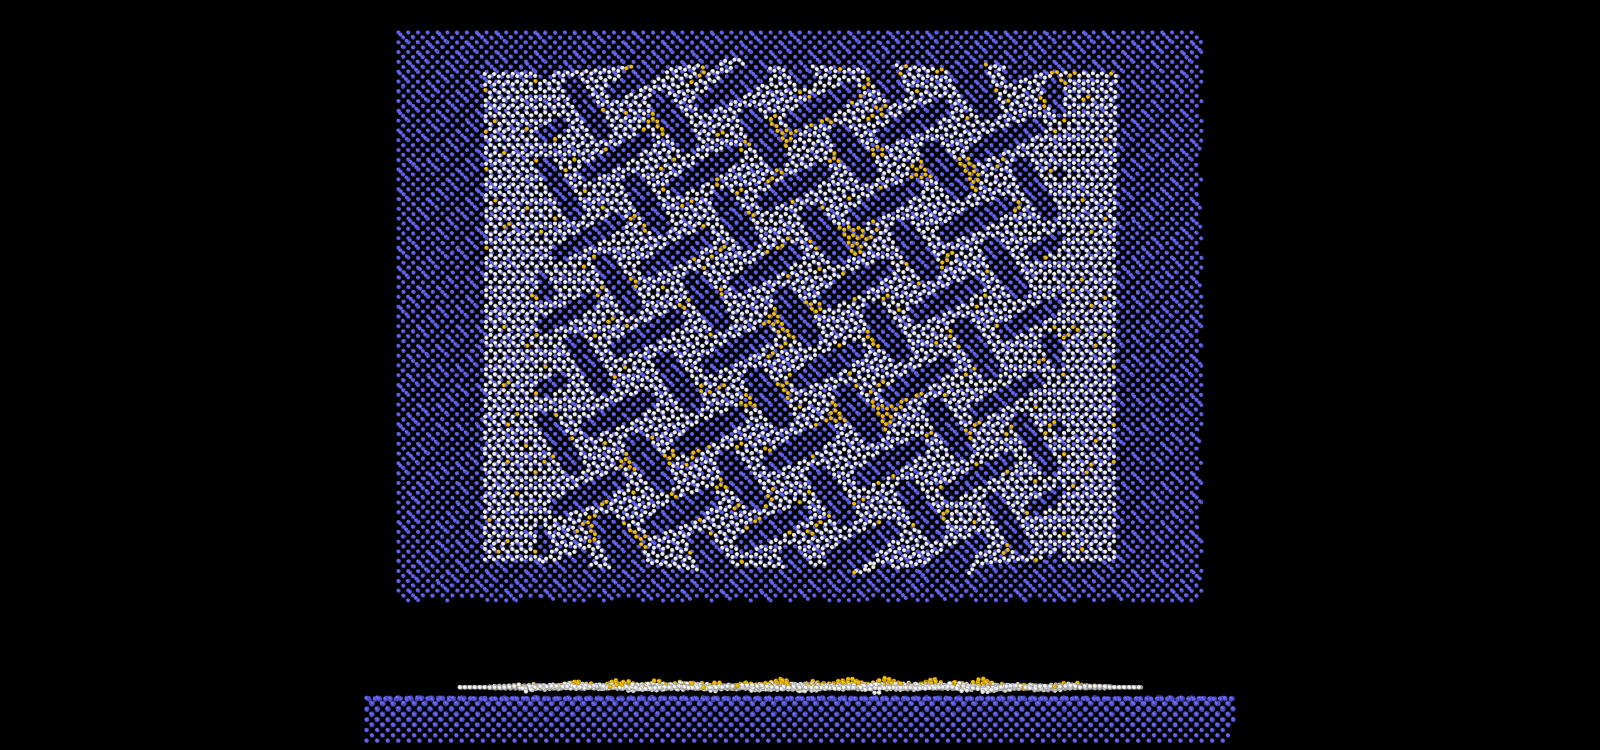
\includegraphics[width=\textwidth]{figures/baseline/contact_vs_stretch/popup/pop_stretch0008.png}
        \caption{Stretch = 0.08}
        \label{fig:}
    \end{subfigure}
    \hfill
    \begin{subfigure}[b]{0.49\textwidth}
        \centering
        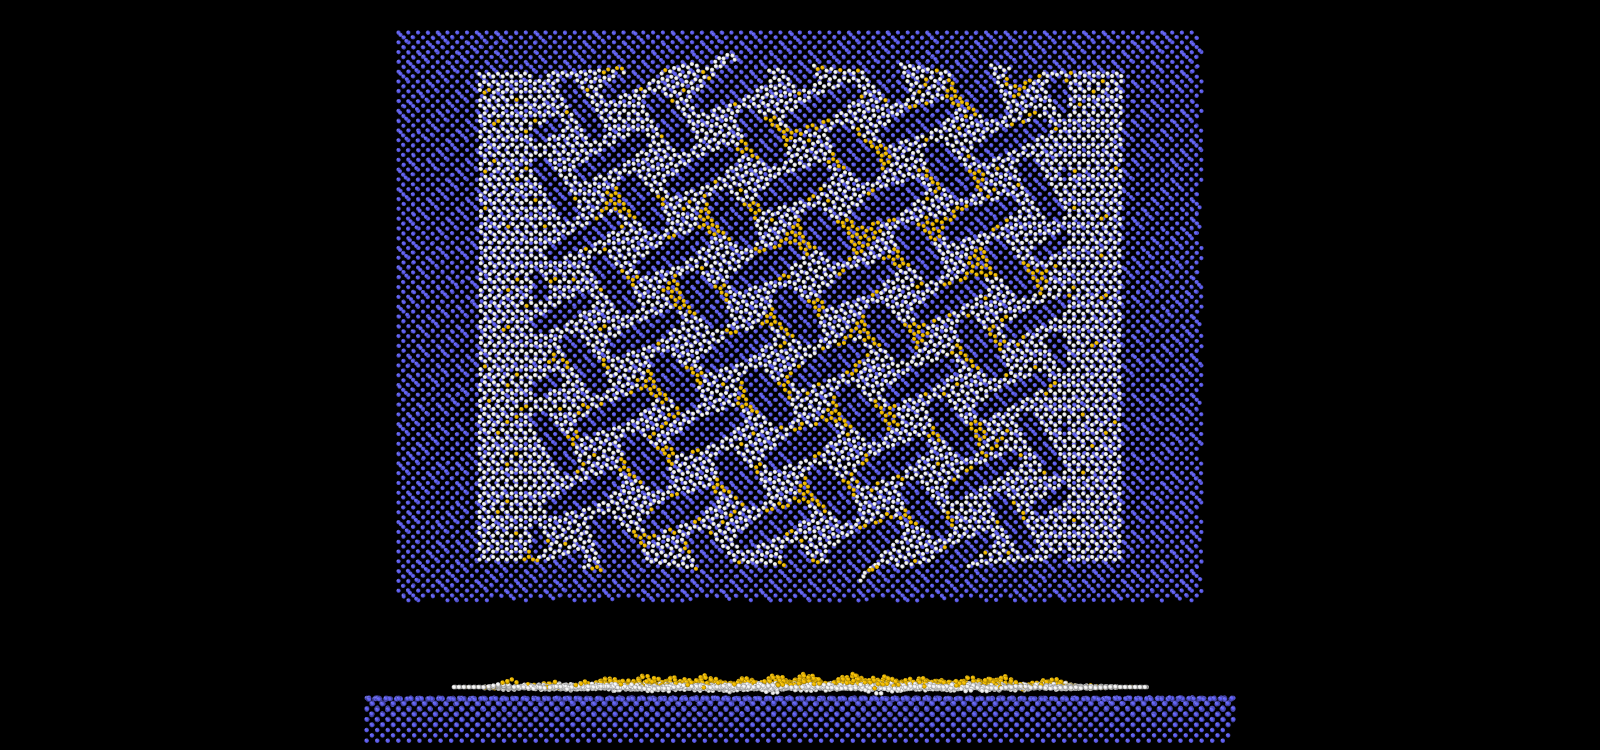
\includegraphics[width=\textwidth]{figures/baseline/contact_vs_stretch/popup/pop_stretch0010.png}
        \caption{Stretch = 0.10}
        \label{fig:}
    \end{subfigure}
    \hfill
    \begin{subfigure}[b]{0.49\textwidth}
        \centering
        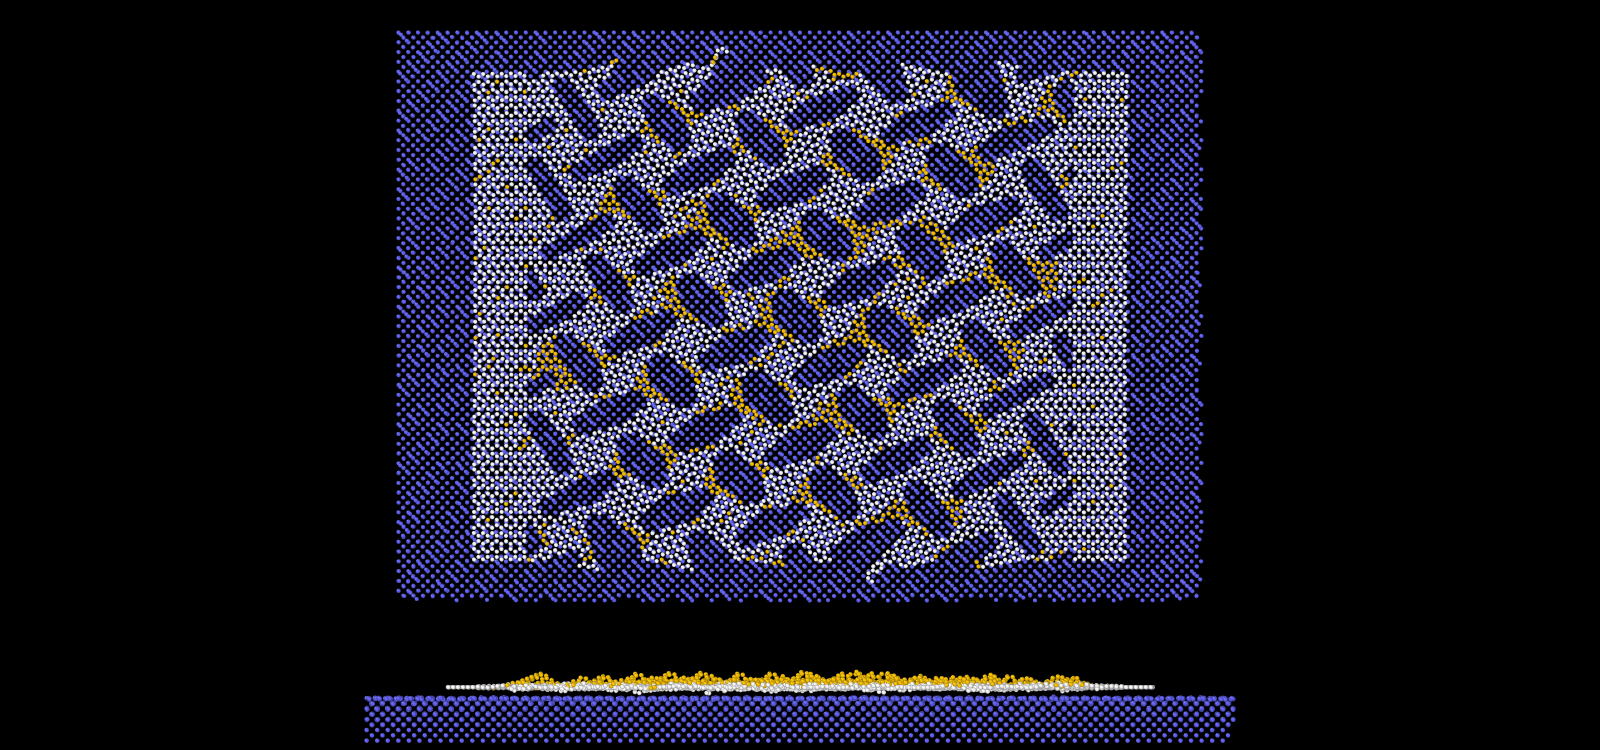
\includegraphics[width=\textwidth]{figures/baseline/contact_vs_stretch/popup/pop_stretch0012.png}
        \caption{Stretch = 0.12}
        \label{fig:}
    \end{subfigure}
    \hfill
    \begin{subfigure}[b]{0.49\textwidth}
        \centering
        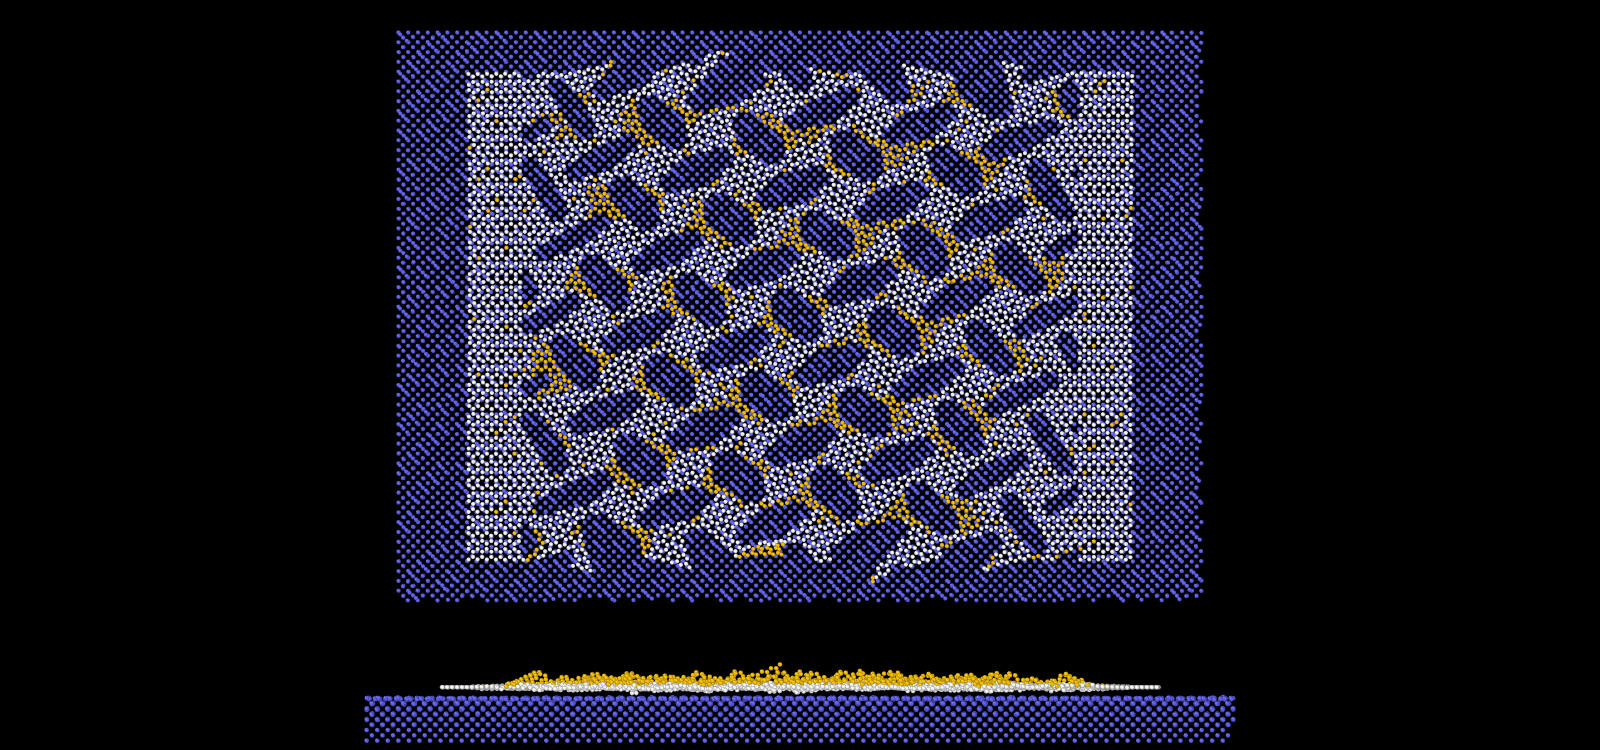
\includegraphics[width=\textwidth]{figures/baseline/contact_vs_stretch/popup/pop_stretch0014.png}
        \caption{Stretch = 0.14}
        \label{fig:}
    \end{subfigure}
    \begin{subfigure}[b]{0.49\textwidth}
        \centering
        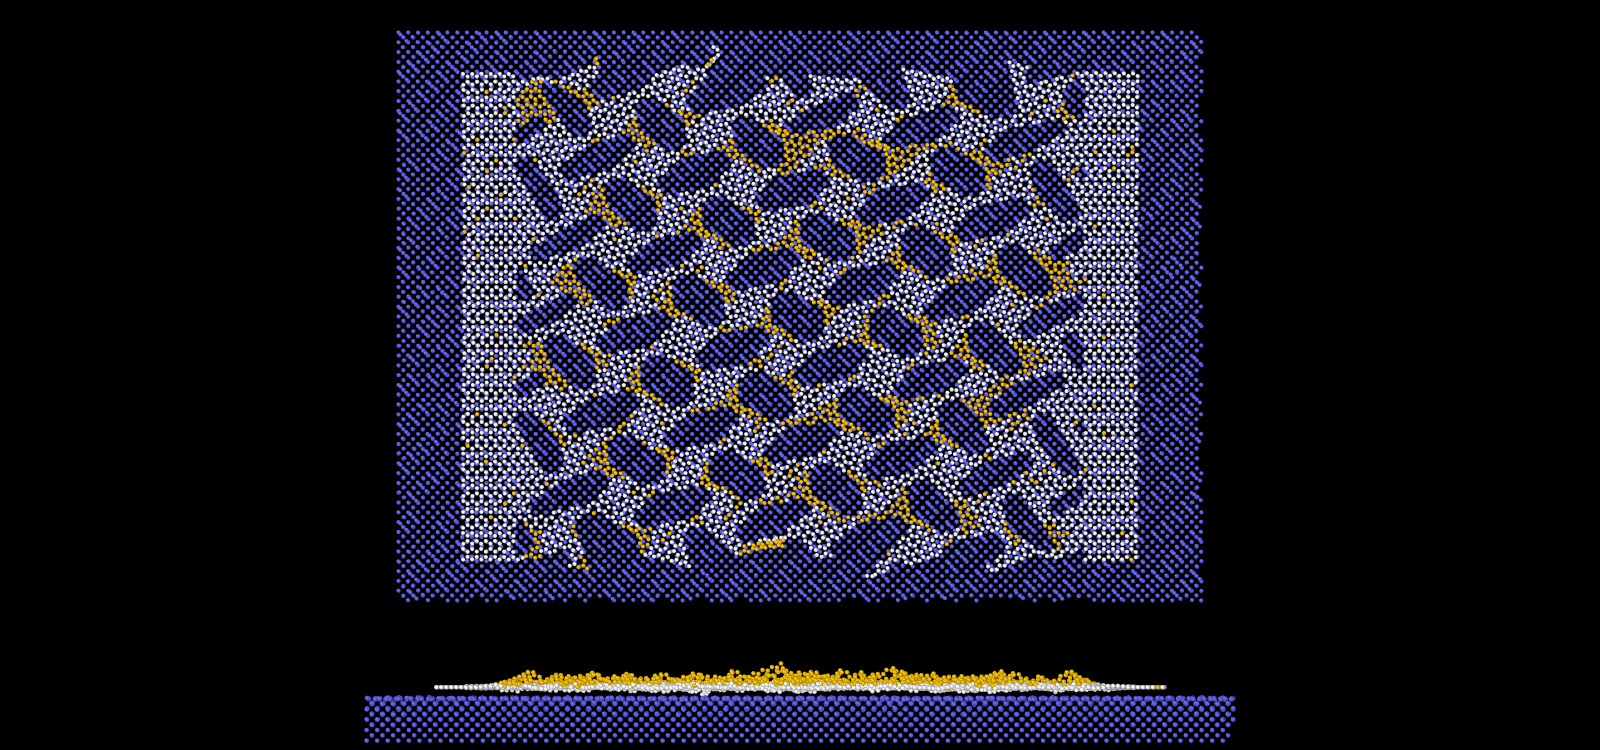
\includegraphics[width=\textwidth]{figures/baseline/contact_vs_stretch/popup/pop_stretch0016.png}
        \caption{Stretch = 0.16}
        \label{fig:}
    \end{subfigure}
    \hfill
    \begin{subfigure}[b]{0.49\textwidth}
        \centering
        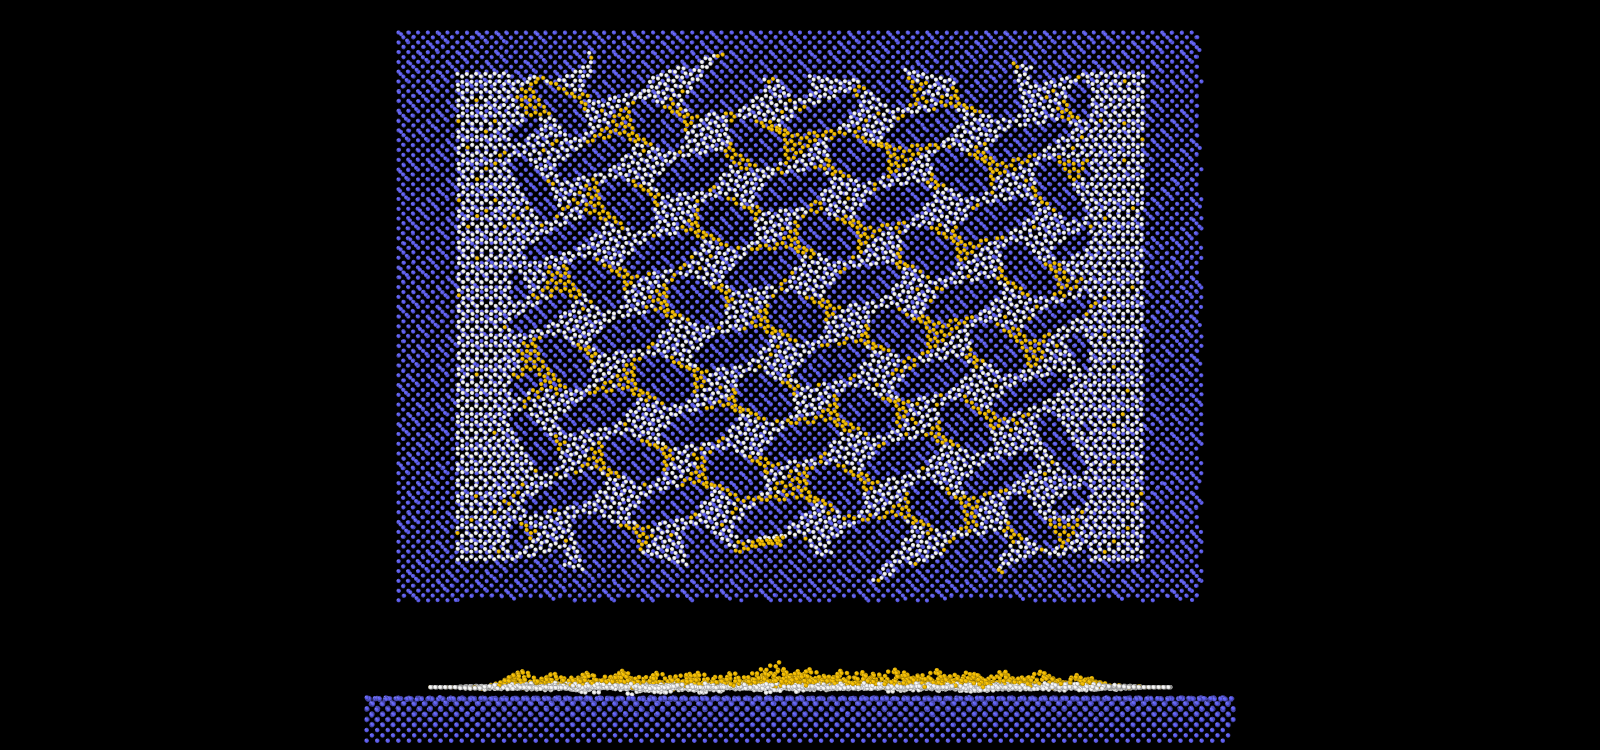
\includegraphics[width=\textwidth]{figures/baseline/contact_vs_stretch/popup/pop_stretch0018.png}
        \caption{Stretch = 0.18}
        \label{fig:}
    \end{subfigure}
    \begin{subfigure}[b]{0.49\textwidth}
        \centering
        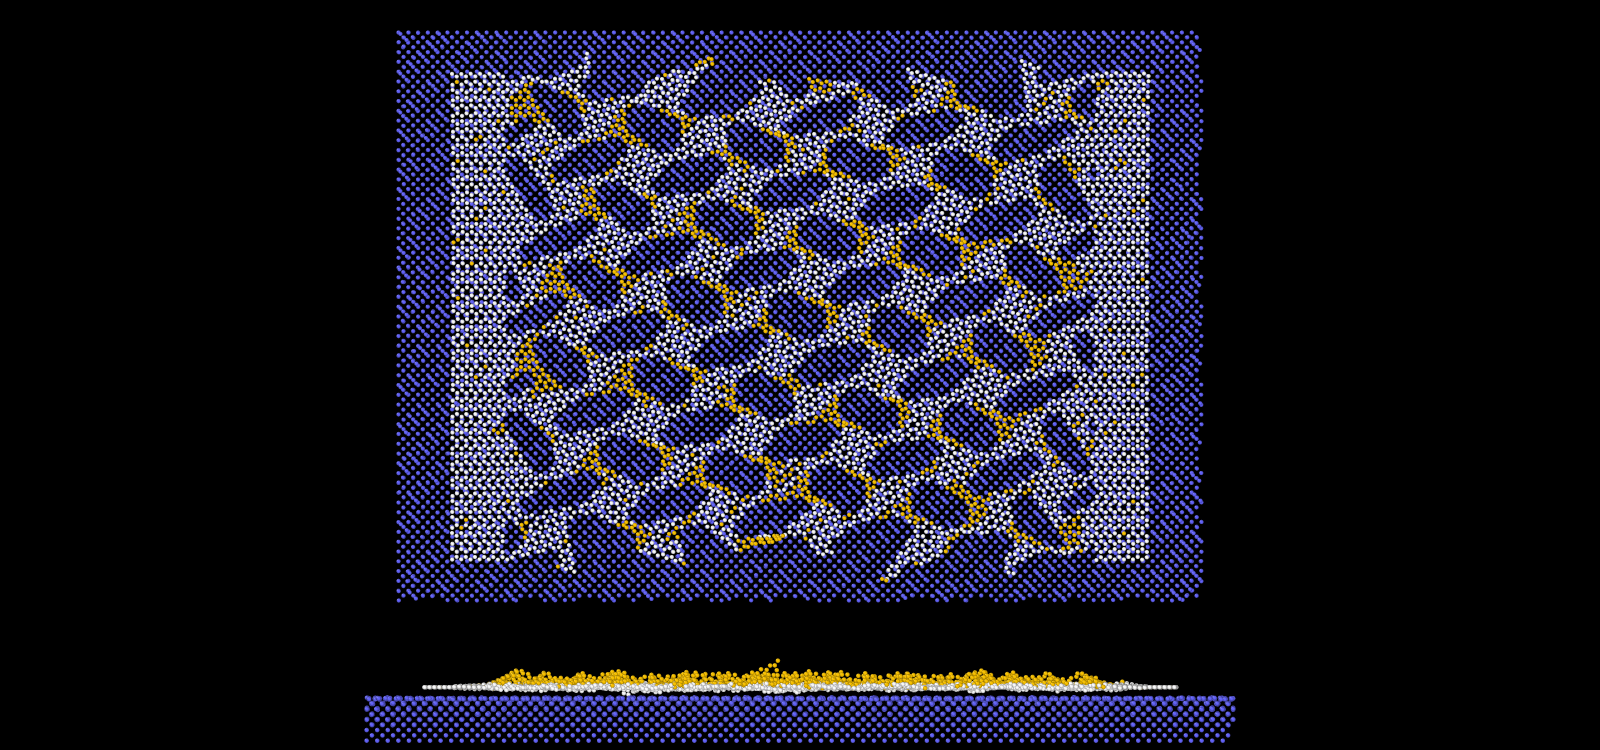
\includegraphics[width=\textwidth]{figures/baseline/contact_vs_stretch/popup/pop_stretch0020.png}
        \caption{Stretch = 0.20}
        \label{fig:}
    \end{subfigure}
    \begin{subfigure}[b]{0.49\textwidth}
        \centering
        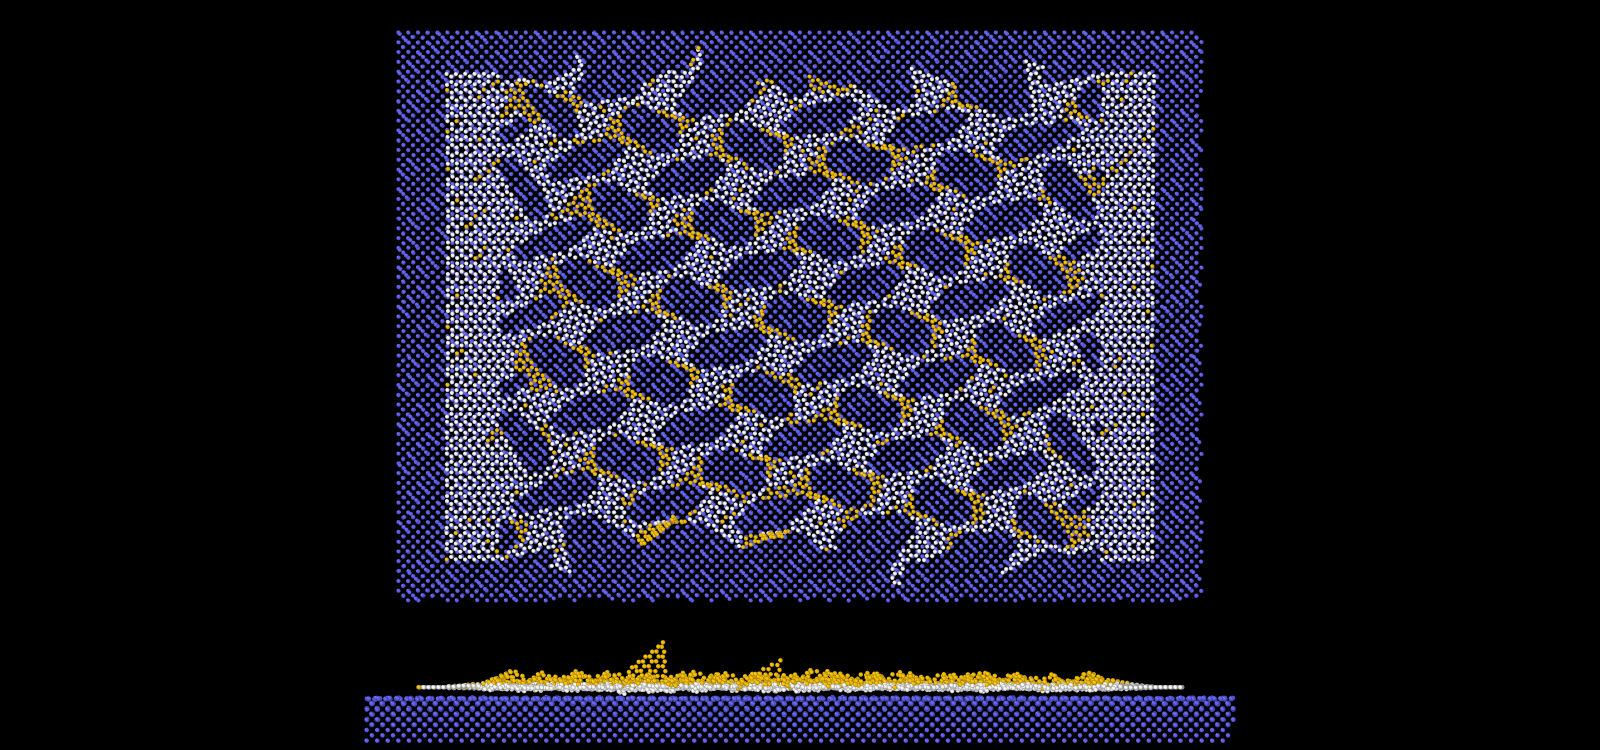
\includegraphics[width=\textwidth]{figures/baseline/contact_vs_stretch/popup/pop_stretch0022.png}
        \caption{Stretch = 0.22}
        \label{fig:}
    \end{subfigure}
    \hfill
       \caption{Stretch of pop-up pattern against substrate. Top part of each frame (a)-(j) shows a top-down view with axis (y, x), and the bottom part shows a side-view with axis (y, z). White colored atoms indicate graphene sheet carbon atoms in contact with the substarte while the yellow colored atoms is not in contact.}
       \label{fig:}
  \end{figure}

% Honeycomb (contact)
\begin{figure}[H]
    \centering
    \begin{subfigure}[b]{0.49\textwidth}
        \centering
        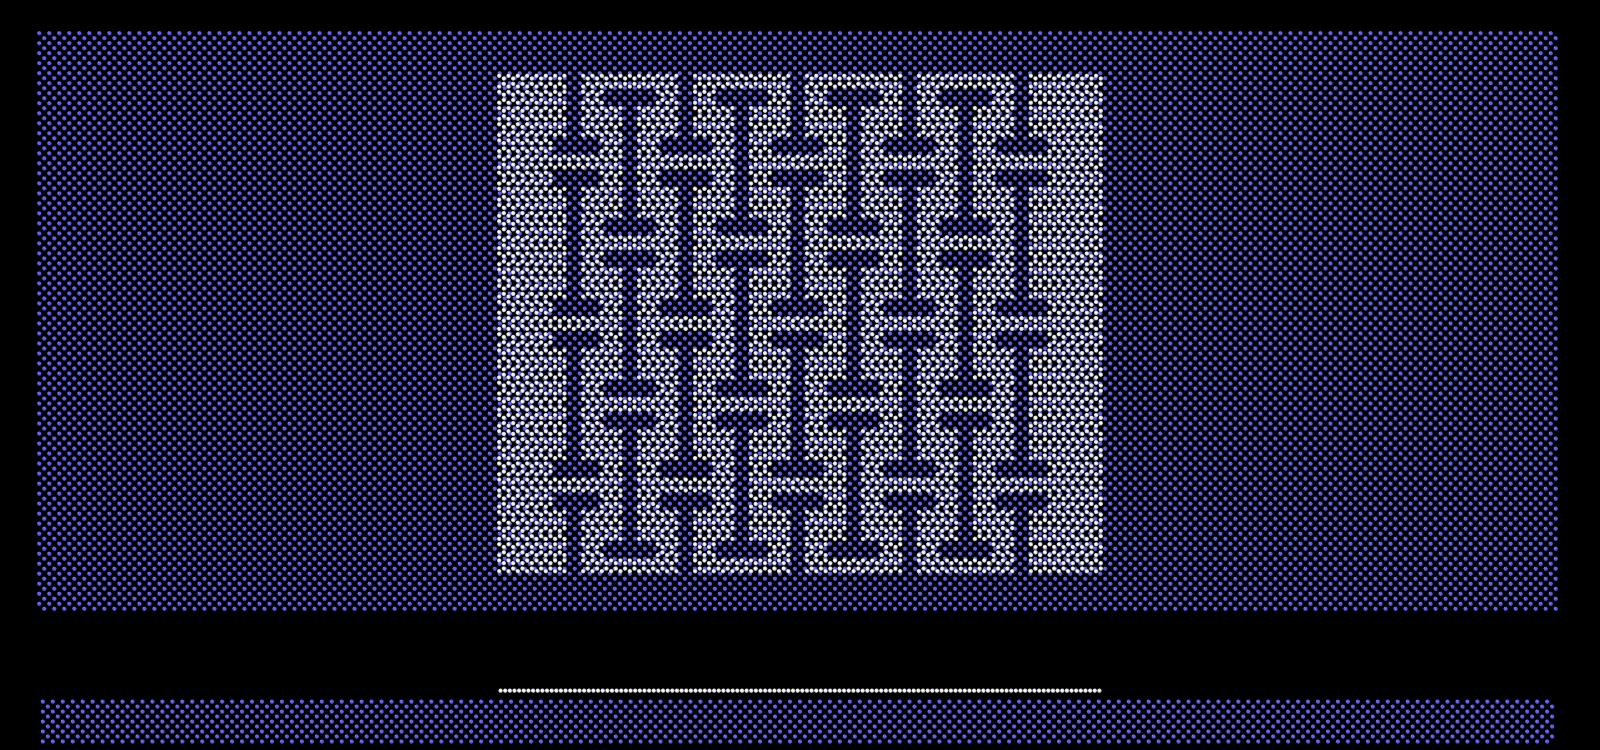
\includegraphics[width=\textwidth]{figures/baseline/contact_vs_stretch/honeycomb/hon_stretch0000.png}
        \caption{Stretch = 0.00}
        \label{fig:}
    \end{subfigure}
    \hfill
    \begin{subfigure}[b]{0.49\textwidth}
        \centering
        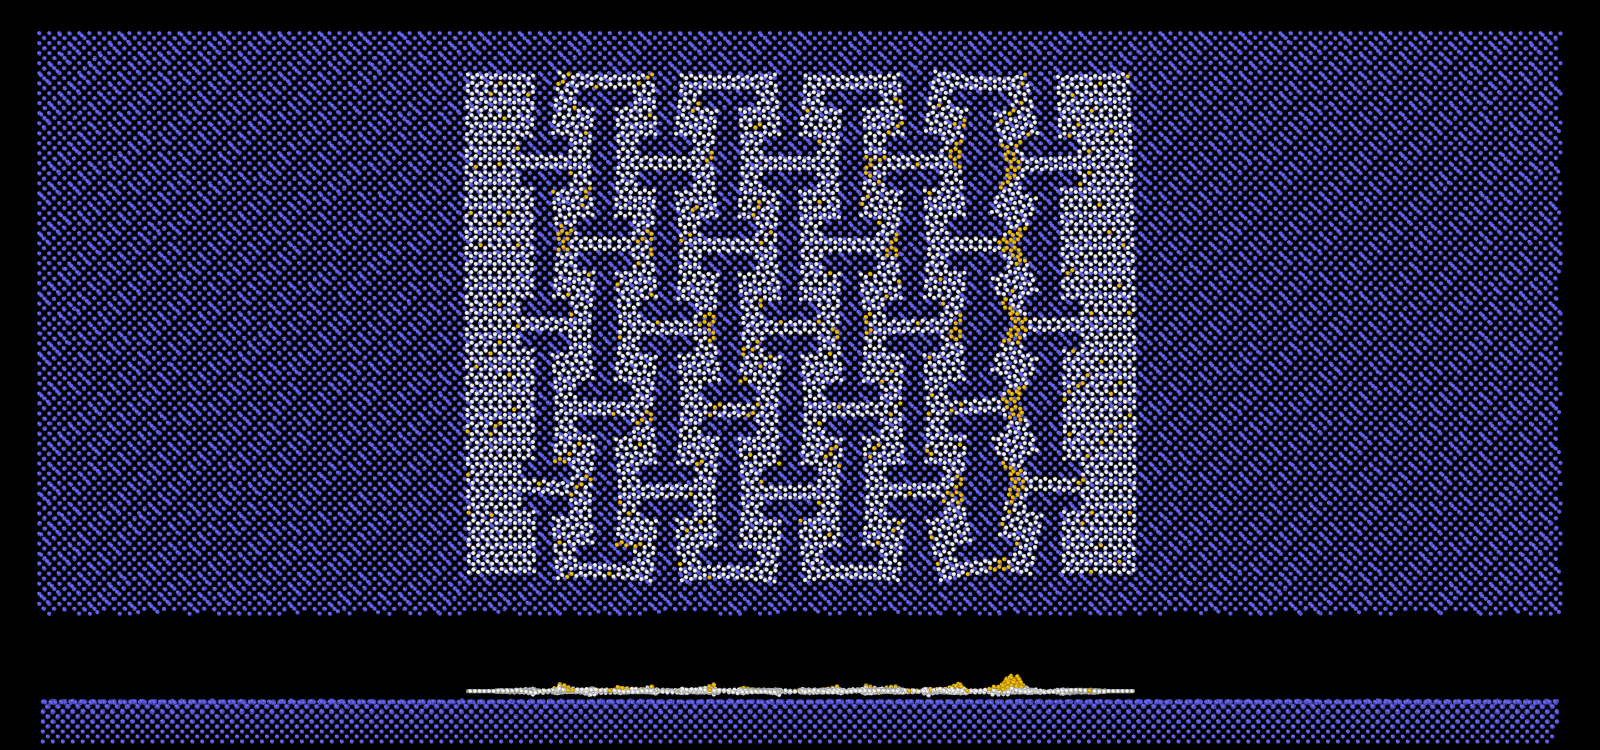
\includegraphics[width=\textwidth]{figures/baseline/contact_vs_stretch/honeycomb/hon_stretch0014.png}
        \caption{Stretch = 0.14}
        \label{fig:}
    \end{subfigure}
    \begin{subfigure}[b]{0.49\textwidth}
        \centering
        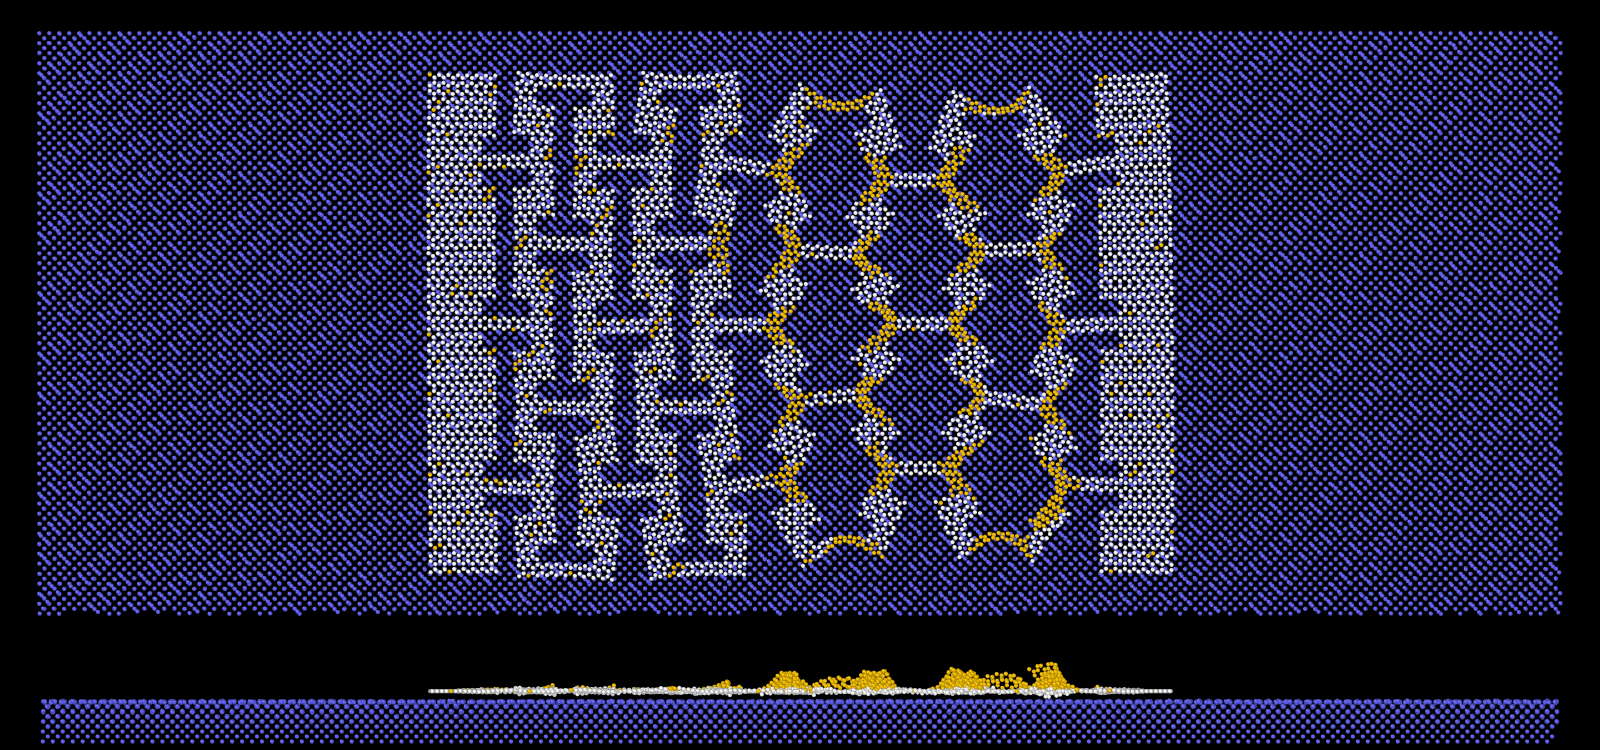
\includegraphics[width=\textwidth]{figures/baseline/contact_vs_stretch/honeycomb/hon_stretch0028.png}
        \caption{Stretch = 0.28}
        \label{fig:}
    \end{subfigure}
    \hfill
    \begin{subfigure}[b]{0.49\textwidth}
        \centering
        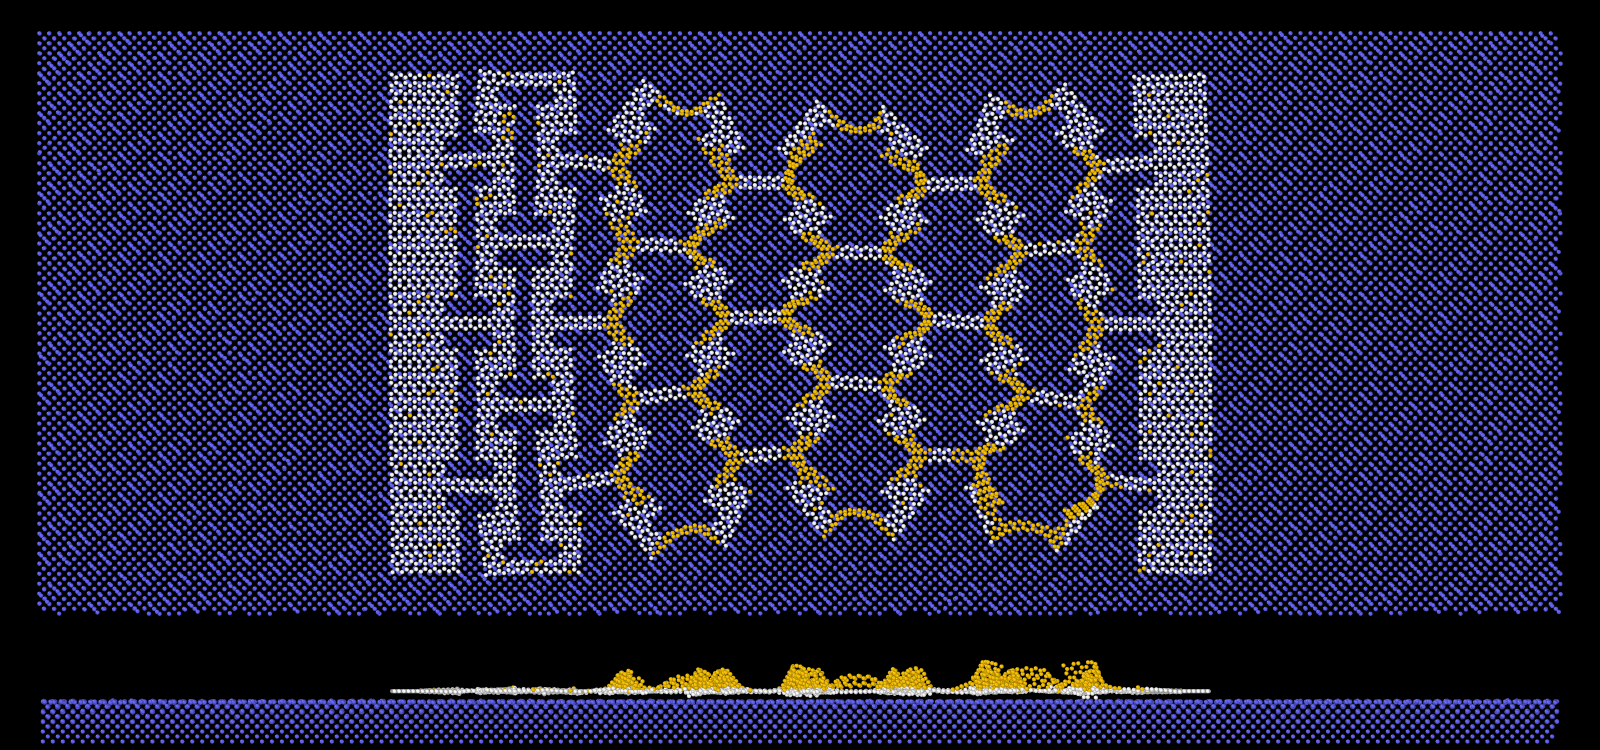
\includegraphics[width=\textwidth]{figures/baseline/contact_vs_stretch/honeycomb/hon_stretch0042.png}
        \caption{Stretch = 0.42}
        \label{fig:}
    \end{subfigure}
    \hfill
    \begin{subfigure}[b]{0.49\textwidth}
        \centering
        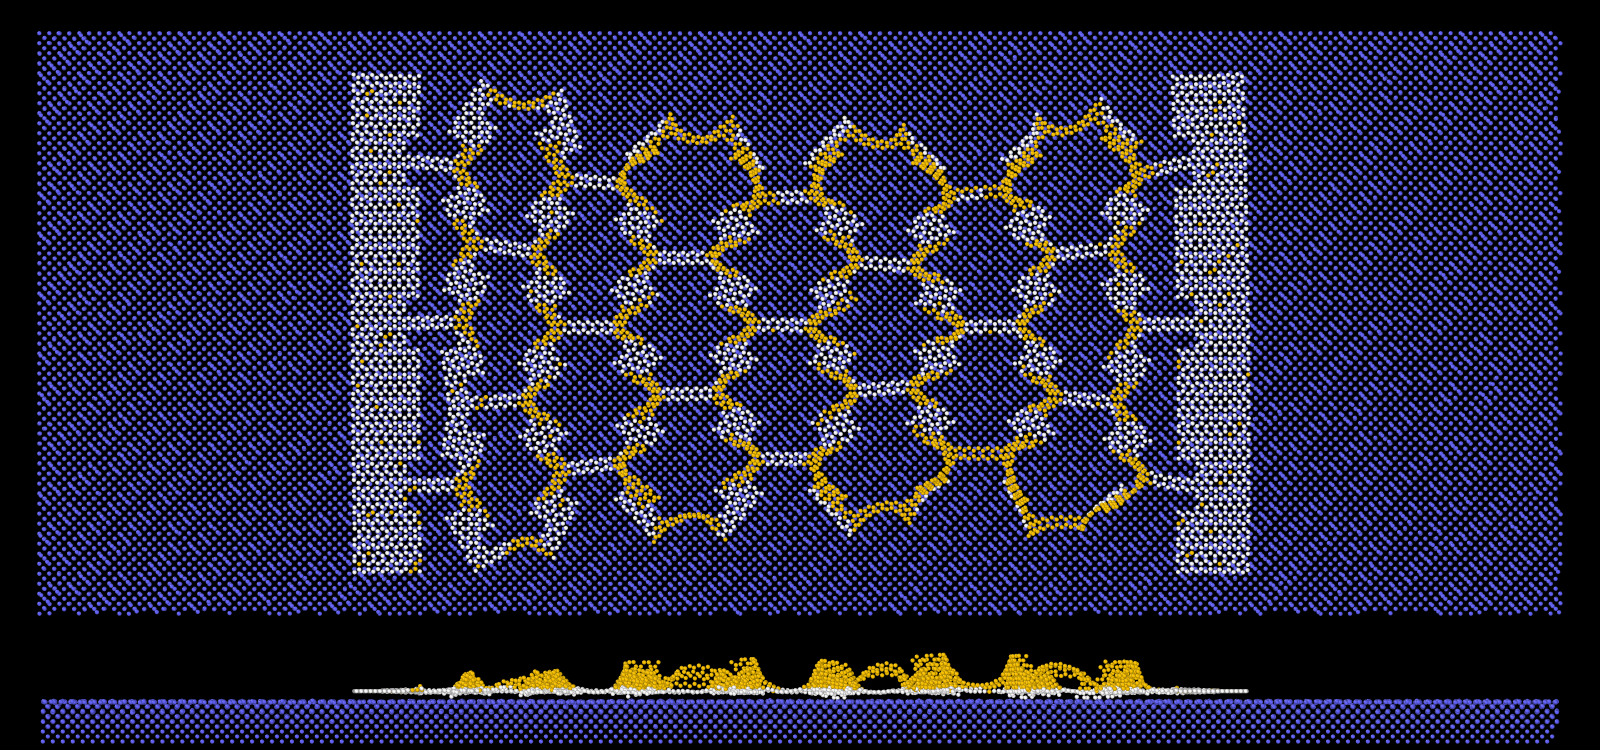
\includegraphics[width=\textwidth]{figures/baseline/contact_vs_stretch/honeycomb/hon_stretch0056.png}
        \caption{Stretch = 0.56}
        \label{fig:}
    \end{subfigure}
    \hfill
    \begin{subfigure}[b]{0.49\textwidth}
        \centering
        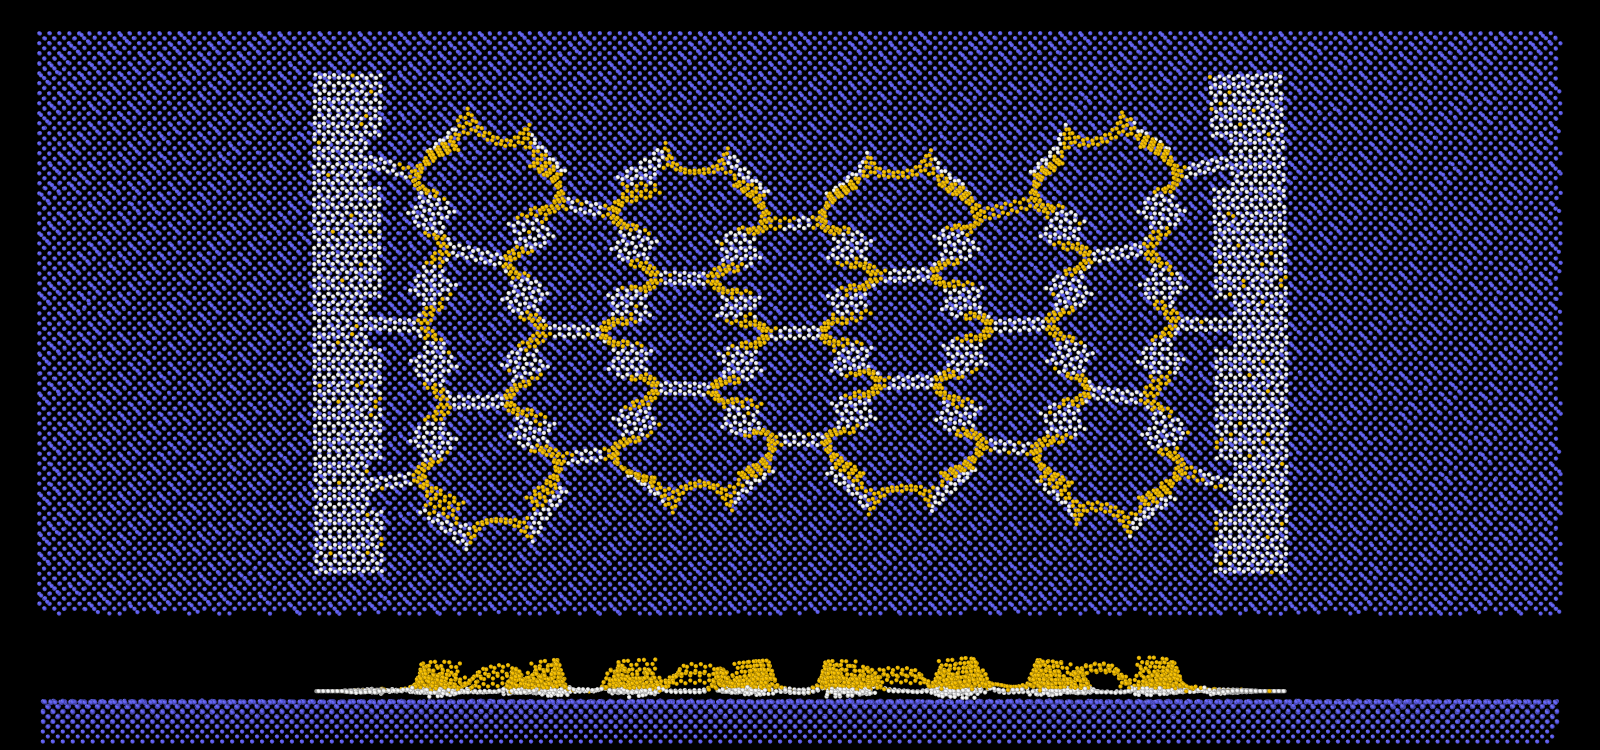
\includegraphics[width=\textwidth]{figures/baseline/contact_vs_stretch/honeycomb/hon_stretch0070.png}
        \caption{Stretch = 0.70}
        \label{fig:}
    \end{subfigure}
    \begin{subfigure}[b]{0.49\textwidth}
        \centering
        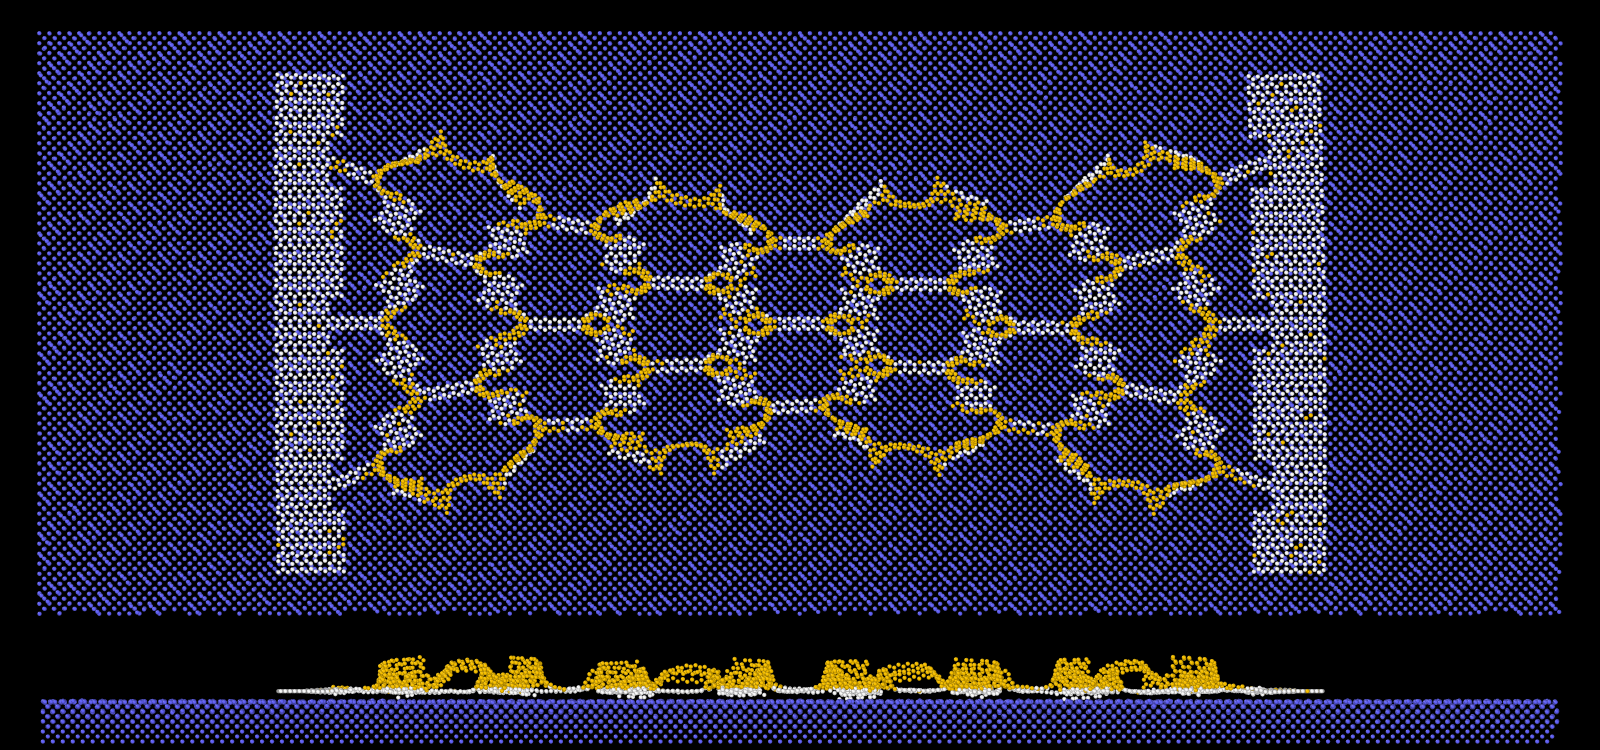
\includegraphics[width=\textwidth]{figures/baseline/contact_vs_stretch/honeycomb/hon_stretch0084.png}
        \caption{Stretch = 0.84}
        \label{fig:}
    \end{subfigure}
    \hfill
    \begin{subfigure}[b]{0.49\textwidth}
        \centering
        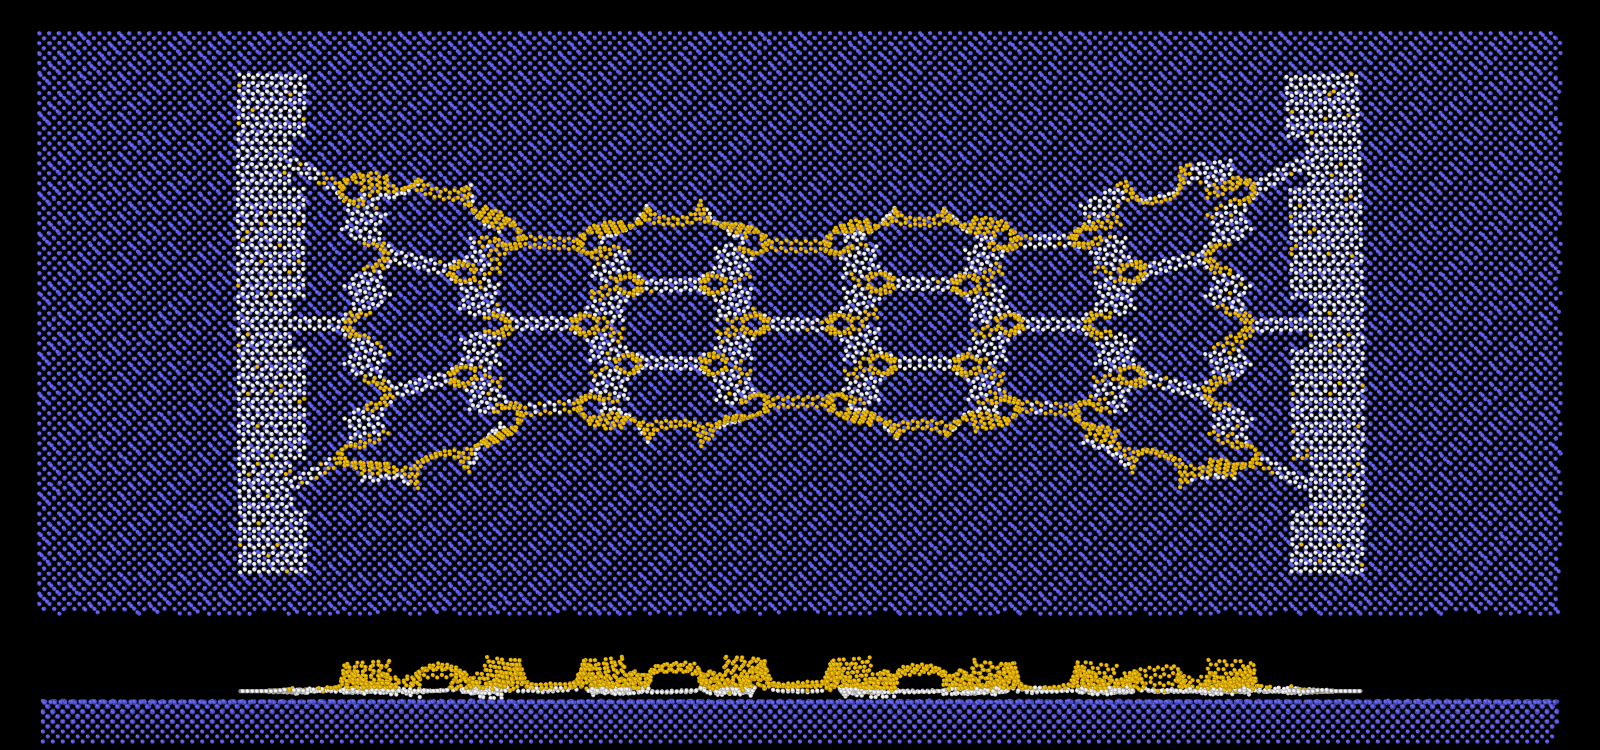
\includegraphics[width=\textwidth]{figures/baseline/contact_vs_stretch/honeycomb/hon_stretch0098.png}
        \caption{Stretch = 0.98}
        \label{fig:}
    \end{subfigure}
    \begin{subfigure}[b]{0.49\textwidth}
        \centering
        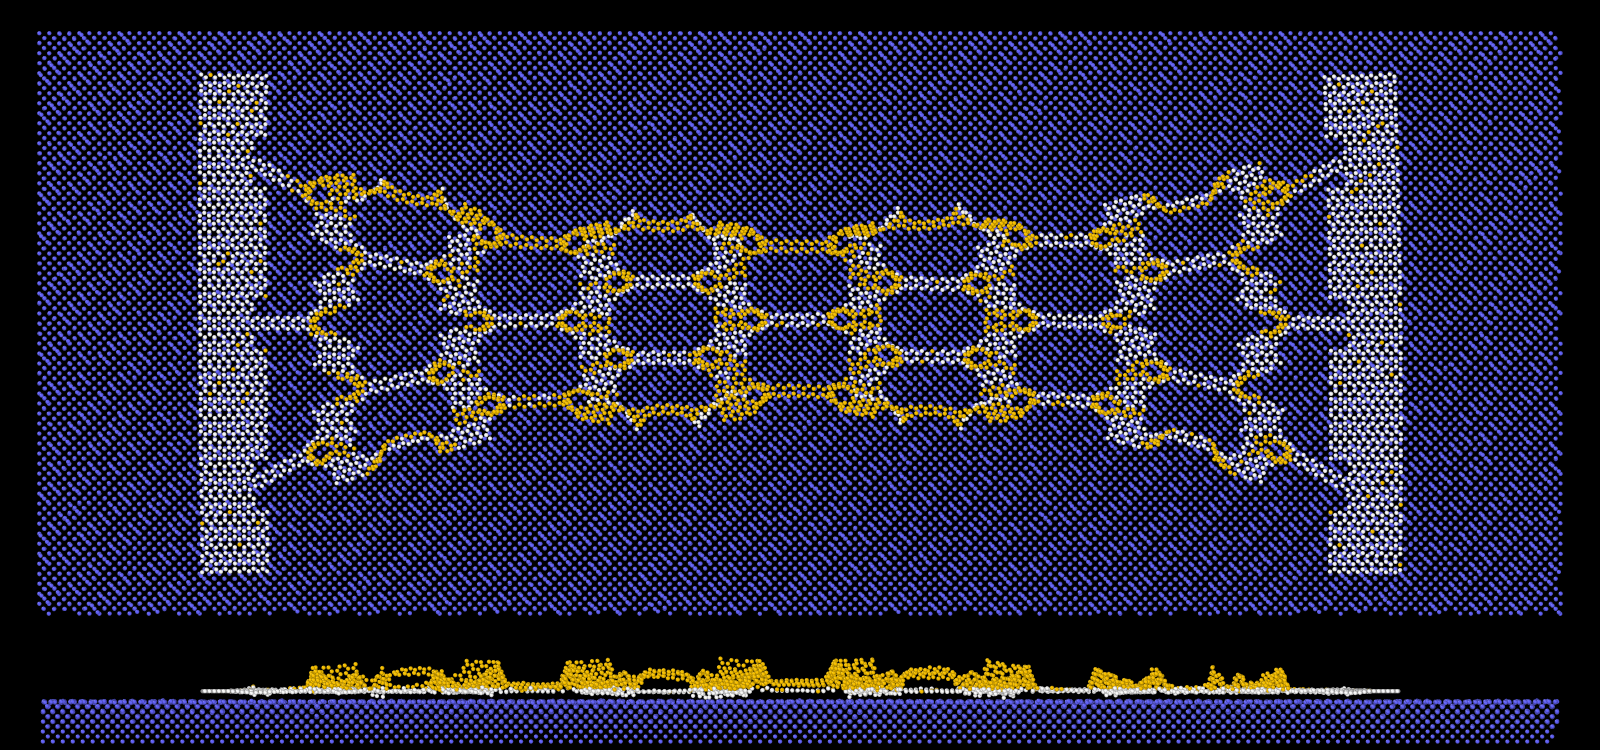
\includegraphics[width=\textwidth]{figures/baseline/contact_vs_stretch/honeycomb/hon_stretch0112.png}
        \caption{Stretch = 1.12}
        \label{fig:}
    \end{subfigure}
    \begin{subfigure}[b]{0.49\textwidth}
        \centering
        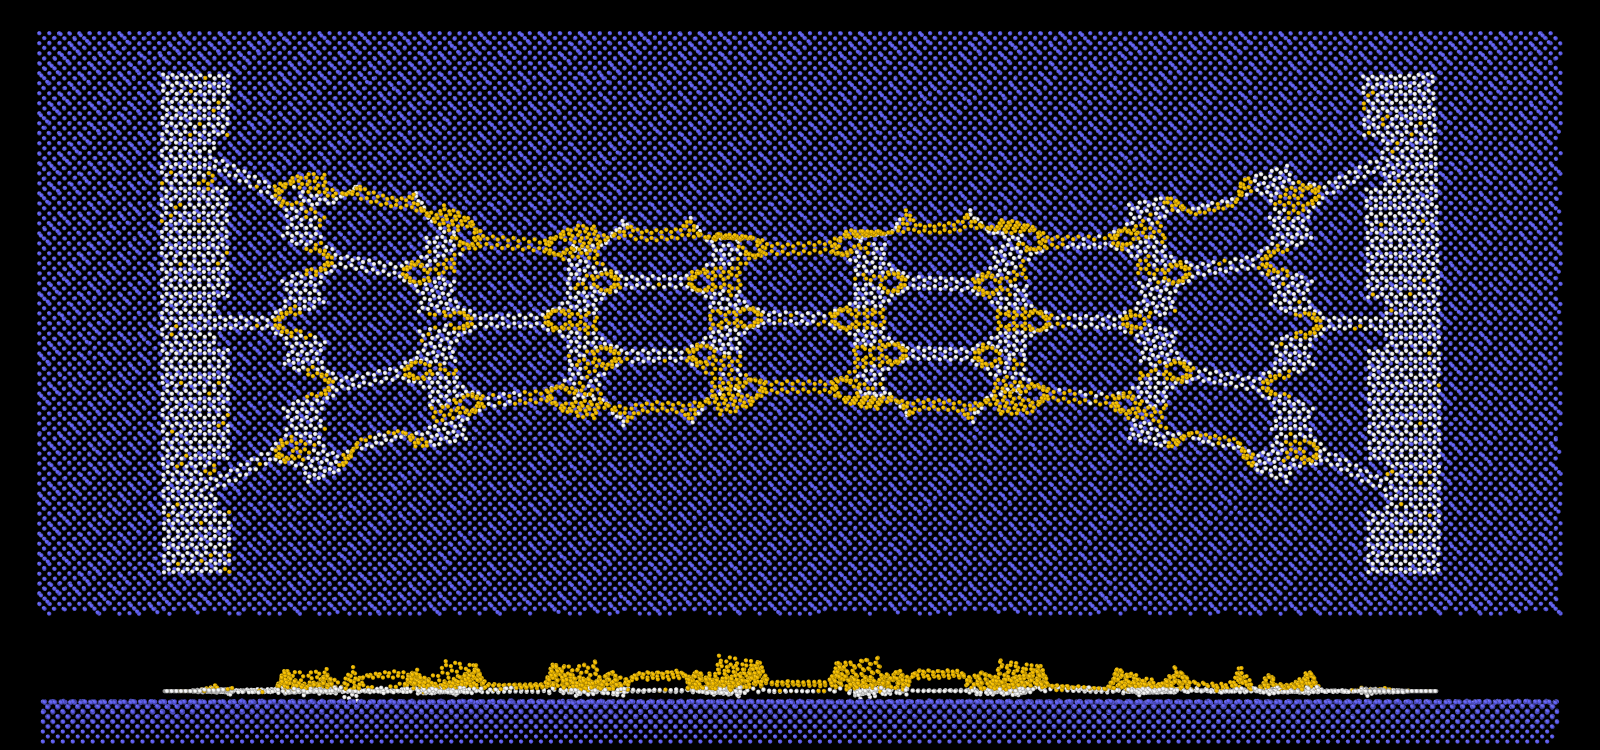
\includegraphics[width=\textwidth]{figures/baseline/contact_vs_stretch/honeycomb/hon_stretch0126.png}
        \caption{Stretch = 1.26}
        \label{fig:}
    \end{subfigure}
    \hfill
       \caption{Stretch of honeycomb pattern against substrate. Top part of each frame (a)-(j) shows a top-down view with axis (y, x), and the bottom part shows a side-view with axis (y, z). White colored atoms indicate graphene sheet carbon atoms in contact with the substarte while the yellow colored atoms is not in contact.}
       \label{fig:}
  \end{figure}
  



  

